\documentclass[12pt]{article}% 这是主要的格式。
\usepackage[UTF8]{ctex}
\usepackage[page,title,titletoc,header]{appendix} 
\usepackage{enumerate}
\usepackage{amsmath}
\usepackage{graphicx}
\usepackage[labelsep=space]{caption}
\usepackage{cite}
\usepackage{textcomp}
\usepackage{array}
\usepackage{bigstrut}
\usepackage{geometry}
\usepackage{graphicx}  
\usepackage{subcaption}
\usepackage{xcolor}  
\usepackage{listings}  
\usepackage{color}  
\usepackage[framed,numbered,autolinebreaks,useliterate]{mcode}
\geometry{left =2.5 cm,right=2.5cm,top=2.5cm,bottom=2.5cm}
\usepackage[section]{placeins}
\usepackage[colorlinks,linkcolor=black,citecolor=black]{hyperref}
\usepackage{titlesec}  
\usepackage{titletoc}
\usepackage[framed,numbered,autolinebreaks,useliterate]{mcode}
\titleformat{\section}{\centering\heiti\zihao{4}}{\thesection}{0.3em}{}
\titleformat{\subsection}{\heiti \fontsize{12pt}{0}}{\thesubsection}{0.3em}{}
\renewcommand\figurename{\heiti\zihao{5} 图}
\renewcommand\tablename{\heiti\zihao{5} 表}

\title{ \heiti\zihao{3}水面舰艇防御鱼雷问题}
\author{}
\date{}

\begin{document}
\section{问题重述}
\subsection{问题的背景}
世界各国军事水平的不断提高,使得水面舰艇对水下自导鱼雷攻击的防御及鱼雷针对舰艇可能采取的反应做出的预判成为海战中的一项重要研究对象。

水面舰艇对抗鱼雷的过程一般是舰艇机动和对鱼雷的拦截两种措施配合实施。舰艇的机动方案优化计算在鱼雷防御方案计算中至关重要,其原则是:
\begin{enumerate}[1)]\addtolength{\itemsep}{-1.5ex}
\item 通过变速、转向以及同时变速和转向,尽可能避免被鱼雷自导装置捕获,捕获区域范围可表示为半径为$d_s$和扇面半角为$\lambda$的扇形区;
\item 尽量远离鱼雷搜索扇面,降低被捕获的可能性;
\item 在不能避免被被捕获的情况下,尽量延缓被捕获的时间,以便尽最大可能地消耗鱼雷航程,为舰艇的成功防御争取机会。
\end{enumerate}
结合表\ref{tab:addlabel1}-表\ref{tab:addlabel2}的相关信息,建立数学模型,回答以下问题。
\subsection{需要解决的问题}

\begin{enumerate}\addtolength{\itemsep}{-1.5ex}

\item 若鱼雷按照正常的提前角—指鱼雷根据和目标相遇的条件计算的提前角度—进行攻击,考虑实战中舰艇对鱼雷自导作用距离的估计有误差及鱼雷后续可能进行的机动搜索,只考虑转向机动,设计合理的舰艇防御机动方案优化指标,建立舰艇机动方案优化模型,针对表\ref{tab:addlabel3}中所给数据,给出最优方案结果。
\item 考虑鱼雷攻击发射方进行鱼雷攻击提前角计算时,对目标运动要素的估计存在误差,不考虑舰艇防御措施,建立声自导鱼雷攻击最佳攻击提前角的计算模型,并对计算结果进行分析,针对表\ref{tab:addlabel3}和表\ref{tab:addlabel2}所给出的数据,给出计算结果,并对结果进行分析。
\item 考虑舰艇鱼雷报警后可能采取的规避机动策略(转向、加速、转向的同时加速),建立相应的声自导鱼雷攻击提前角优化计算模型,并针对表\ref{tab:addlabel3}和表\ref{tab:addlabel2}给出的数据,给出最优方案结果。
\item 若鱼雷攻击要求捕获目标的概率不小于最小捕获概率$P$,建立鱼雷可攻性判断模型,并针对前述参数,给出可攻性分析结论。
\end{enumerate}
\section{问题分析}
\subsection{问题的重要性分析}
随着各国军事实力的提高,水面舰艇与水下鱼雷间的攻击与防御的博弈将成为未来海战中的重要内容。

水面舰艇对抗鱼雷的过程一般都是舰艇机动和对鱼雷的拦截两种措施配合实施。而随着自导鱼雷的出现,舰艇的机动方案优化计算在鱼雷防御方案计算中至关重要。而面对这些规避方案,鱼雷发射方又该怎样最大程度地发挥鱼雷作用,这都是事关军事国防实力的、需要解决的问题。

\subsection{文献综述}
邹振华,李守奇等通过对水面舰艇规避来袭自导鱼雷过程的分析,对水面舰艇规避鱼雷的基础模型做了一定的探索\cite{1}。董严红,卫翔等则从鱼雷纯方位攻击的角度探讨鱼雷命中概率\cite{3}。 武志东,朱伟良等针对声自导鱼雷直进射击时的射击参数,设计了一种消除系统误差的提前角修正方法\cite{2}。

但大多数同类型的文献,是单独以鱼雷或舰艇作为研究对象,缺少二者间的相互影响作用。
\subsection{问题的思路分析}
\begin{enumerate}[1.]\addtolength{\itemsep}{-1.5ex}
\item 针对问题一,为了尽量不被捕获,应该在鱼雷的6海里可用搜索航程内不被搜索到;考虑到舰艇对鱼雷自导作用距离的估计存在的误差,舰艇的转动时机应当适当提前。
\item 针对问题二,由于测量存在误差,需要进行一定的调整。但事实上每一次发射鱼雷前进行的测量,实际上只能看做是单次测量。对于单次测量带来的误差,在已知均方差的情况下进行修正。
\item 针对问题三,对问题一的模型进行适当的修改,通过合理的方法给出加速、转向、转向同时加速相应的约束函数,结合问题二的模型,对提前角做出进一步的优化。
\item 针对问题四,需要给出捕获目标的概率,和要求的最小概率比较来建立可攻性判断模型。结合问题三中给出的模型,做出可攻性判断分析。
\end{enumerate}
\section{问题假设}
为了简化模型同时更好地进行分析,我们做出如下假设:
\begin{enumerate}[1.]\addtolength{\itemsep}{-1.5ex}
\item 假定舰艇每次只需要躲避一颗鱼雷,即不存在多颗鱼雷攻击同一舰艇的情况;
\item 假设一旦进入舰艇、鱼雷的探测范围后,舰艇或鱼雷能立刻发现敌方,并立刻做出反应,即不存在延迟时间。且,假设鱼雷做出转动时不产生转动半径,即假设鱼雷可以就地完成转动;
\item 为了更好地描述模型,以舰艇所在位置为原点,建立直角坐标系,假设舰艇最初沿正北方向并设其为X轴正方向,设正西方向为Y轴正方向;
\item 假设舰艇驾驶人员在操作舰艇时不存在失误,即所有指令均能被极好地执行;
\item 假设舰艇在不进行操作时能恰好保持原来的运动状态,鱼雷在捕获舰艇之前按直线前进,不考虑水流、引力等因素对运动状态的影响;
\item 假设舰艇、鱼雷均可看作质点;
\item 假设题中所有数据真实可靠。
\end{enumerate}
\section{符号说明}
\begin{table}[htbp]
  \centering
    \begin{tabular}{c|c}
    \hline
    符号 & 解释说明 \\
      \hline
    $P(t):(P_x(t),P_y(t))$  & t时刻舰艇位置 \\
      \hline
      $Q(t):(Q_x(t),Q_y(t))$ &t时刻鱼雷位置 \\
            \hline
      $d(t)$ &t时刻舰艇与鱼雷距离 \\
            \hline
      $R_s$ &舰艇的探测距离 \\
            \hline
      $d_s$ &鱼雷的探测距离 \\
            \hline
      $\lambda$ &鱼雷搜索区域扇面半角\\    
        \hline
      $X$ &以舰艇为基准,对鱼雷的舷角 \\
         \hline
      $\phi(t)$ &以鱼雷为基准,对舰艇的舷角\\
         \hline
      $H_L$ &鱼雷的航向\\
         \hline
      $H$ &舰艇的航向\\
         \hline
               $V_l$ &鱼雷的速度\\
         \hline
               $V_m$ &舰艇的速度\\
         \hline
         $\varphi$ &提前角\\
            \hline
                  $s$ &冲矩\\
         \hline
                        $R$ &舰艇的转向半径\\
         \hline
    \end{tabular}%
  \label{tab:addlabel}%
\end{table}%

\onecolumn
\section{模型的建立及求解}
\subsection{模型一:基于迭代思想的舰艇躲避模型}
模型的建立:

针对问题一,结合假设,给出舰艇、鱼雷情况大致示意图如图\ref{fig:label1}。
\begin{figure}[htb]
\centering
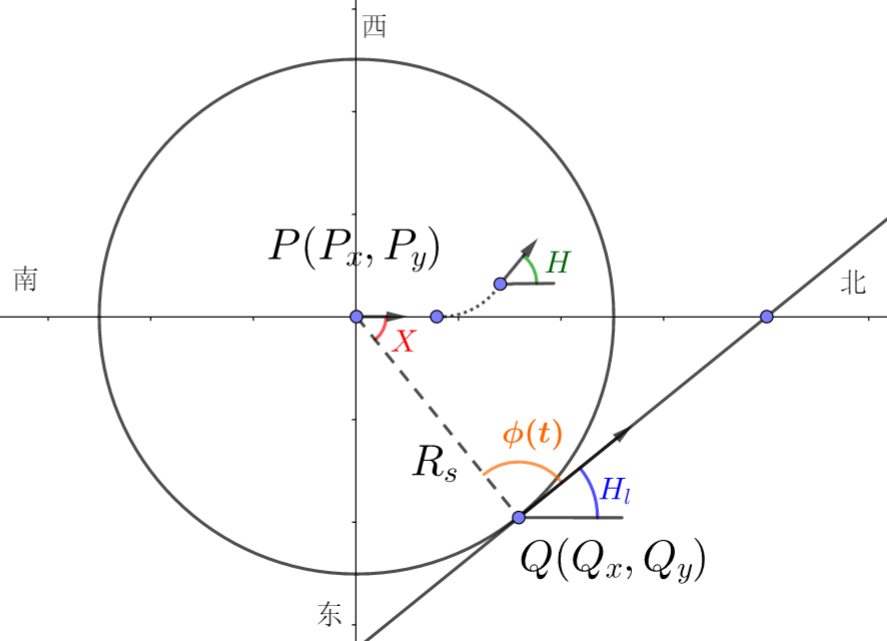
\includegraphics[width=10cm]{TIM20180526232647.png}
\caption{\zihao{5}\heiti 舰艇、鱼雷情况大致示意图}
\label{fig:label1}
\end{figure}
记$P(t)=(P_x(t),P_y(t))$为舰艇任意时刻的坐标位置,$P(0)=(0,0)$;$Q(t)=(Q_x(t),Q_y(t))$为鱼雷任意时刻坐标位置。则二者距离$d$的表达式为:
\begin{equation}\label{juligongshi1}
d(t)=\sqrt{(P_x(t)-Q_x(t))^{2}+(P_y(t)-Q_y(t))^2}
\end{equation}
设0时刻舰艇发现鱼雷,即$d(0)=R_s$,$R_s$为舰船对鱼雷的探测距离。
则鱼雷0时刻坐标满足:
$\left\{ 
\begin{array}{c}
Q_x(0)= R_scos(|X|) \\
Q_y(0)=R_ssin(|X|)
\end{array} \right.  $,
其中$X$为以舰艇为基准时,对鱼雷的舷角。

记t时刻,鱼雷航向为$H_l(t)$,则
鱼雷在捕获目标前的位置情况满足:
\begin{equation}\label{yuleiweizhi}
\left\{ 
\begin{array}{c}
Q_x(t)=Q_x(0)+V_ltcos(H_l)\\
Q_y(t)=Q_y(0)+V_ltsin(H_l) 
\end{array} \right.  
\end{equation}
其中$V_l$为鱼雷的速度。

舰艇被鱼雷捕获的条件为:
\begin{equation}\label{buhuotiaojian}
\left\{ 
\begin{array}{c}
d_s\ge d(t)  \\
\lambda \ge| \phi(t)|
\end{array} \right.  
\end{equation}
其中,$d_s$为鱼雷对舰艇的探测距离,$\lambda$为鱼雷搜索扇面半角,$\phi(t)$为以鱼雷为基准时,对舰艇的舷角。$\phi(t)$满足:
\begin{equation}\label{jiao}
\phi(t)=arccos\left(\frac{\vec V_l\bullet \overrightarrow{QP}}{|V_l|\bullet|d(t)|}\right)
\end{equation}
进入捕获范围后,鱼雷的速度方向调整为指向
舰艇位置,即满足:
\begin{equation}\label{jiantingweizhi}
\vec V_l = \overrightarrow{QP} \Leftrightarrow H_l=arctg\frac{P_y-Q_y}{P_x-Q_x}
\end{equation}
以上是整个过程中鱼雷的运动情况讨论,对于舰艇的情况,我们分析如下:

任意时刻,舰艇有3种操作可供执行:顺时针转向、逆时针转向及直行。\\
对于直行,其航向$H$不改变,位置变化满足:
\begin{equation}\label{jiantingzhiweizhi}
\left\{ 
\begin{array}{c}
P_x=V_m\Delta tcosH +P_{x0}\\
P_y=V_m\Delta tsinH+P_{y0}
\end{array} \right. 
\end{equation}
其中,$V_m$为舰艇的速度,$P_{x0},P_{y0}$为进行直行操作前的P坐标。

对于顺、逆时针转向,只是方向不同,以顺时针为例,其航向满足:
\begin{equation}\label{jiantinghangxiang}
H=\frac{V_m}{R}\Delta t+H_0
\end{equation}
其中,$H_0$为顺时针转向前的航向,R为转动半径。舰艇的位置变化的求解参照图\ref{fig:label2},满足:

\begin{figure}[htb]
\centering
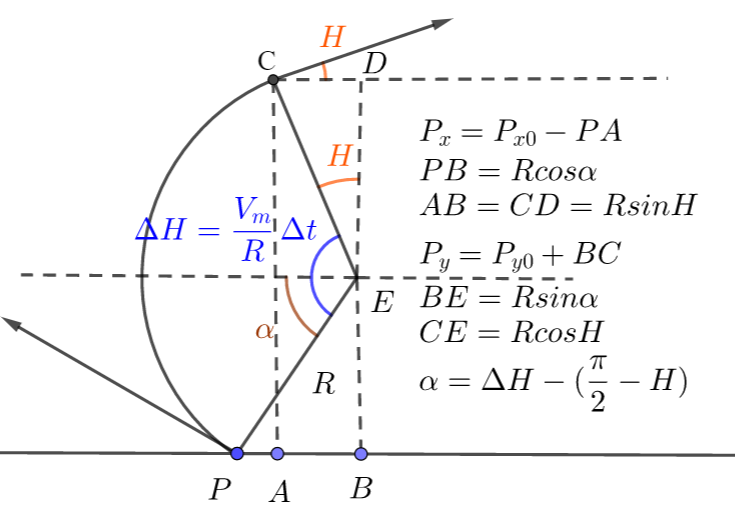
\includegraphics[width=12cm]{TIM20180527231733.png}
\caption{\zihao{5}\heiti 舰艇顺时针转动参数关系图}
\label{fig:label2}
\end{figure}
\begin{equation}\label{jiantingzhuanweizhi}
\left\{ 
\begin{array}{c}
P_x=P_{x0}-Rcos\left(\frac{V_m}{R}\Delta t-\frac{\pi}{2}+H\right)+R\Delta tsinH\\
P_y=P_{y0}+Rsin\left(\frac{V_m}{R}\Delta t-\frac{\pi}{2}+H\right)+R\Delta tcosH
\end{array} \right. 
\end{equation}
其中,$P_{x0},P_{y0}$为进行顺时针转动操作前的P坐标。

逆时针的情况相同,只需要将$V_m$变为$-V_m$即可。

综合以上的分析,给出舰艇的总变化情况方程:
\begin{equation}\label{jiantingzongfangcheng}
\left\{ 
\begin{array}{c}
H_n=K_1(\frac{V_m}{R}\Delta t+H_{n-1})\\
P_{xn}=P_{x(n-1)}+K_1(Rsin\left(\frac{K_2V_m}{R}\Delta t+H_n\right)+R\Delta tsinH)+(K_1-1)(V_m\Delta tcosH_n)\\
P_{yn}=P_{y(n-1)}+K_1(Rcos\left(\frac{K_2V_m}{R}\Delta t+H_n\right)+R\Delta tcosH)+(K_1-1)(V_m\Delta tsinH_n)
\end{array} \right. 
\end{equation}
其中涉及到2个选择变量,分别是转动选择变量$K_1(\in \{0,1\})$,确定舰艇是否转动,0时为直行,1时为转动;方向选择变量$K_2(\in\{-1,+1\})$,确定转动的方向,1为顺时针,-1为逆时针。借助$K_1,K_2$的不同取值,可以实现对舰艇不同运动状态下的运动情况分析。

至此,鱼雷与舰艇的运动情况分析完成,得到关于舰艇、鱼雷航向与位置的,以时间为变量的多个模型函数。\\\ \\
模型的求解:

对于得到的模型,需要考虑的变量较多,我们做出一定简化:考虑极端情况,显然,鱼雷初始发射位置越靠近舰艇,留给舰艇的反应时间越短,鱼雷的实际有效可用航程也越接近6海里。由此我们认为$\phi(0)=\varphi=arcsin\left(\frac{V_m}{V_l}sinX\right)$;而对于其他的变量,基于迭代思想,为了避免复杂的判断,我们先行随机产生大量的、符合参数所在范围的参数值以及各种操作方案,模拟各种舰艇规避鱼雷的可能情况,代入到模型中,结合题中所给的规避原则,我们认为一旦舰艇被鱼雷捕获,则这种方案在一定情况下失效。通过大量的假设来弥补已知条件的不足,借助迭代思想直接判断方案可行度。

为了得出比较优化的方案,以减少实际操作中驾驶人员可能存在失误为考量,我们以\textcolor{red}{操作数}作为舰艇防御机动方案优化指标,即认为,需要进行的变动越少越好、越简单越好(出错的概率越小)。

但当带入MATLAB进行迭代时,我们发现,基于这个模型,即便是$n=1$的情况,仍然有很多数量的方案可供选择。因此,我们给出舰艇防御机动方案的第二个优化指标——\textcolor{red}{时间},即保证操作足够简单的情况下,越快逃离越好。最终的方案对于不同的X所决定的不同位置的鱼雷,有不同的转角,给出结果如下:\\
当X$<\frac{3\pi}{10}$,需要转动的转角较小$\theta<\frac{3\pi}{10}$\\
当$\frac{3\pi}{10}<X<\frac{\pi}{2}$,需要转动的转角较大$\theta>\frac{\pi}{2}$\\
当$X>\frac{\pi}{2}$,需要转动的转角又变小$\theta<\frac{\pi}{2}$。
\subsection{模型二:提前角优化模型}
模型的建立:

针对问题二,误差的来源是发射平台对于目标的距离、舷角、速度大小的测量误差。这些误差分别服从正态分布。由题中所给的原提前角计算公式
\begin{equation}\label{tiqianjiao}
\varphi=arcsin\left(\frac{V_m}{V_l}sinX\right)
\end{equation}
可知,鱼雷与目标当前距离D对鱼雷可用航程产生影响,但对提前角的计算并不起影响作用,而。因此,对于产生影响的$V_m,X$我们需要稍作修正。

由概率统计相关原理可知,对正态分布而言,处于$[\mu-\sigma ,\mu+\sigma]$范围的频率较高且较为集中,因此我们随机产生n个服从正态分布且在$[\mu-\sigma ,\mu+\sigma]$区间范围内的波动值变量$V_m+\Delta V_m,X+\Delta X$。将随机生成的波动值带入到公式(\ref{tiqianjiao})中,可以得到n个相应的$\varphi$值,将这n个$\varphi$以大小为标准,划分为m组,可以得到各个组别的$\varphi$数量占总数量的分布情况,当n足够大,这个分布情况可以一定程度上反应$\varphi$的概率。
\begin{equation}\label{tiqianjiao2}
\varphi=arcsin\left(\frac{V_m+\Delta V_m}{V_l}sin(X+\Delta X)\right)
\end{equation}\\\ \\
模型的求解:

按照模型的思想,我们利用MATLAB产生随机变量,取$n=1000$,可以得到测得部分舷角X的情况下的$\varphi$值分布,按照不同的打击精度要求,可以选择对应的$\varphi$。
这里给出若干X测量值下的提前角分布情况,见图\ref{fig:label3}
\begin{figure}
	\centering\zihao{5}
	\begin{tabular}{ccc}
		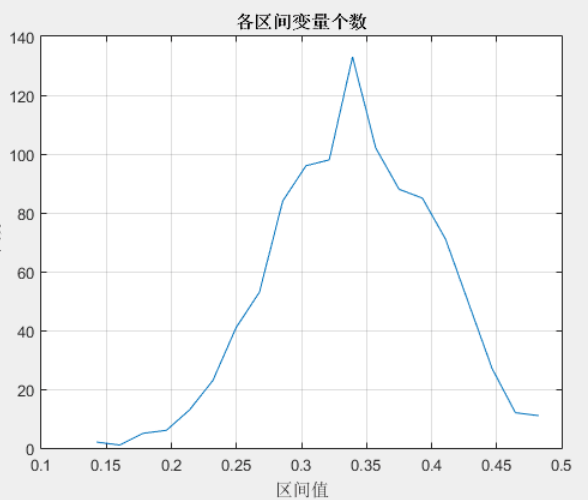
\includegraphics[width=0.33\linewidth]{TIM20180528014501.png}  & 
		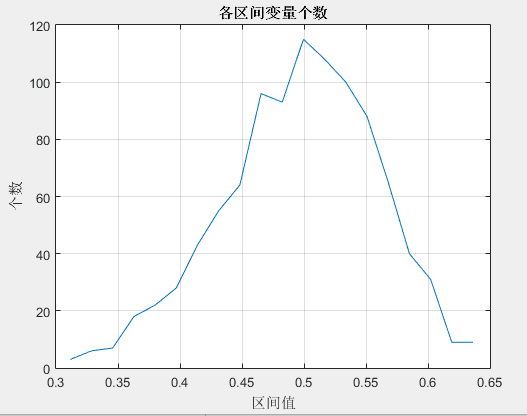
\includegraphics[width=0.33\linewidth]{TIM20180528035003.png}  &
		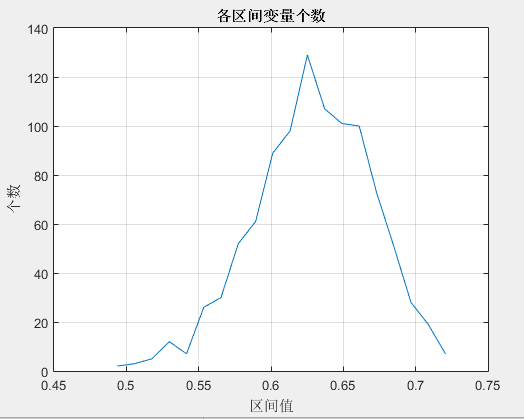
\includegraphics[width=0.33\linewidth]{TIM20180528035052.png} \\
		(a) $\frac{\pi}{6}$时的$\varphi$分布情况 & (b) $\frac{\pi}{4}$时的$\varphi$分布情况&(c) $\frac{\pi}{3}$时的$\varphi$分布情况\\
		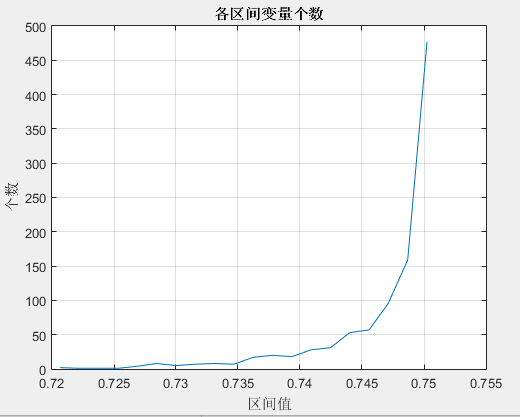
\includegraphics[width=0.33\linewidth]{TIM20180528035131.png}  & 
		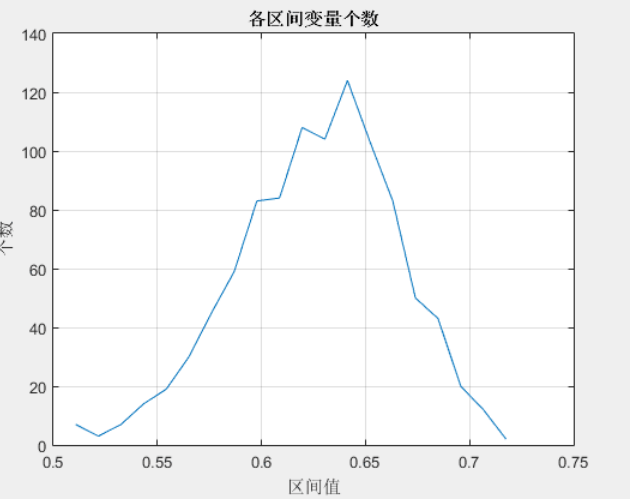
\includegraphics[width=0.33\linewidth]{TIM20180528035205.png}  &
		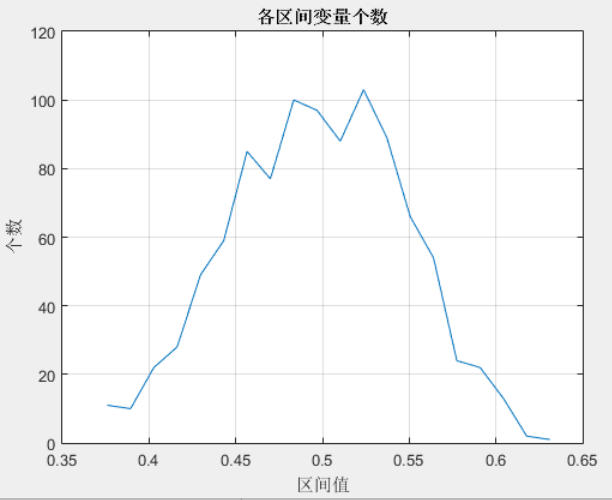
\includegraphics[width=0.33\linewidth]{TIM20180528035239.png} \\
		(d) $\frac{\pi}{2}$时的$\varphi$分布情况 & (e)  $\frac{2\pi}{3}$时的$\varphi$分布情况)&(f) $3\frac{\pi}{4}$时的$\varphi$分布情况\\
			 & 
		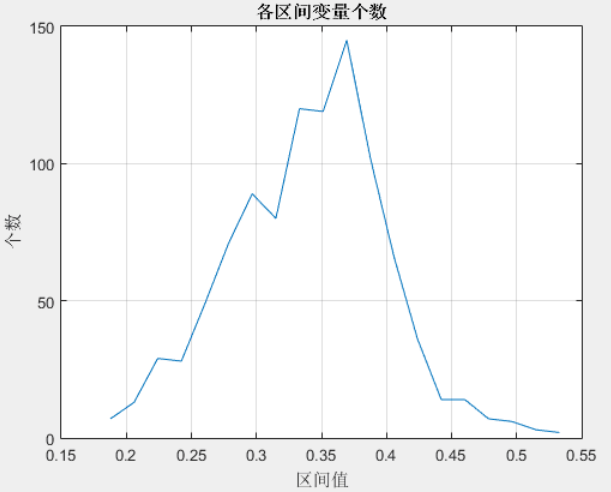
\includegraphics[width=0.33\linewidth]{TIM20180528035311.png}  &
		 \\
		 		&(g)  $\frac{5\pi}{6}$时的$\varphi$分布情况& \\
	\end{tabular}
	\caption{\zihao{5}\heiti几种舷角X下的$\varphi$分布情况 }
	\label{fig:label3}
	\vspace{-0.5em}
\end{figure}
\subsection{模型三:考虑舰艇规避方案的微分思想提前角优化模型}
模型的准备:

针对问题三,我们需要给出舰艇在加速、转向、加速同时转向的情况下,鱼雷提前角的优化方案。

首先根据给出的舰船加速时间和冲距表计算任意速度变化情况下的加速度、冲矩公式:

分析表中的第1-2组数据,计算起始速度相同时的加速度、冲矩,设$\Delta$为速度变化1节时,对应的加速度变化量、n为速度变化节数、b为加速度修正常数;c为冲距修正常数、Q为节数变化影响因子,得到:
\begin{equation}\label{jiasudu1}
\left\{ 
\begin{array}{c}
a=b+n\Delta \\
s=V_0t+ka^2+c+nQ
\end{array} \right.  
\end{equation}
分析表中第2-3组数据,计算(大致)相同的速度变化量下的加速度、冲矩,设$\Delta V$为速度变化量、N为节数变化快量、$b'$为此时的加速度修正常数;P为速度变化影响因子,得到:
\begin{equation}\label{jiasudu2}
\left\{ 
\begin{array}{c}
a=b'+N\Delta V\\
s=V_0t+ka^2+c+NP
\end{array} \right.  
\end{equation}
将3组数据分别带入公式(\ref{jiasudu1})(\ref{jiasudu2})中,求出相应的参数及影响因子值。
得到如下结论:从22节加速到27节时的a=109.953m/$s^2$,s=3900m;进而得出,从22节加速到任意节数n时的情况。

接下来,需要根据不同航速下舰艇转向半径表确定任意航速下的转向半径。\\借助EXCEL函数拟合,根据麦克劳林展开式原理,以多项式拟合出半径的情况见图\ref{fig:label5}
\begin{equation}\label{1}
R=-0.3886V_m^3+25.628V_m^2-469.74V_m+2917.9
\end{equation}
\begin{figure}[htb]
\centering
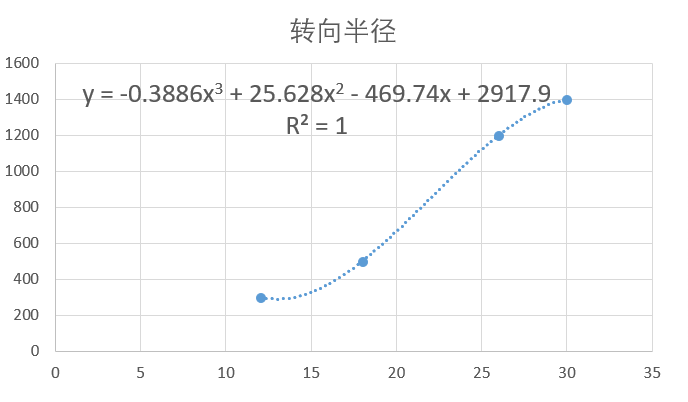
\includegraphics[width=10cm]{TIM20180528164001.png}
\caption{\zihao{5}\heiti 转动半径拟合公式}
\label{fig:label}
\end{figure}

不同鱼雷速度、舰艇速度对舰艇对鱼雷探测距离、鱼雷对舰艇探测距离也有影响,借助EXCEL画出曲面图见图\ref{fig:label6}—\ref{fig:label7}
\begin{figure}[htb]
\centering
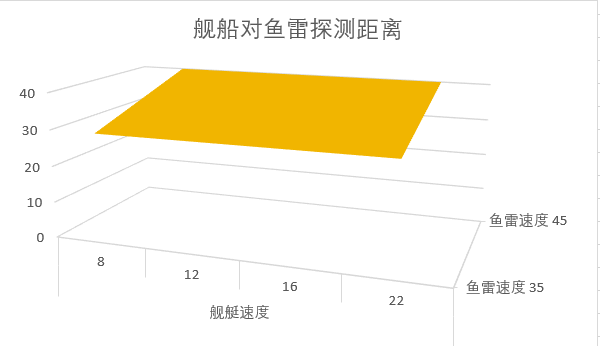
\includegraphics[width=10cm]{TIM20180528164726.png}
\caption{\zihao{5}\heiti 舰艇对鱼雷探测距离受舰艇速度、鱼雷速度影响曲面图}
\label{fig:label6}
\end{figure}
\begin{figure}[htb]
\centering
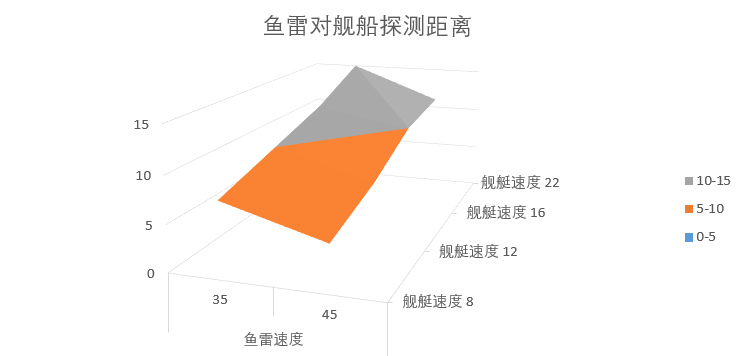
\includegraphics[width=12cm]{TIM20180528165255.png}
\caption{\zihao{5}\heiti 鱼雷对舰艇探测距离受舰艇速度、鱼雷速度影响曲面图}
\label{fig:label7}
\end{figure}


模型的建立:

对于加速同时转向的情况,借助微分思想,认为在极小的$\Delta t$内,速度V不变,则有
\begin{equation}\label{weifen1}
\left\{ 
\begin{array}{c}
V_i=V_{i-1}+\frac{a-b}{i}\\
s_i=V_{i}\Delta t+ka_i^2+c+iQ \\
\frac{s_i}{R_i}=\Delta H_i\\
P_{xi}=P_{x(i-1)}+s_icos\Delta H_i\\
P_{yi}=P_{y(i-1)}+s_isin\Delta H_i\\
\end{array} \right.  
\end{equation}
对于转向的情况则可以套用问题一的模型,结合公式(\ref{jiantingzongfangcheng}),而对于加速的情况,则可以认为是$\Delta H$不发生改变的转动加速
\begin{equation}\label{weifen2}
\left\{ 
\begin{array}{c}
V_i=V_{i-1}+\frac{a-b}{i}\\
s_i=V_{i}\Delta t+ka_i^2+c+iQ \\
P_{xi}=P_{x(i-1)}+s_icosH_i\\
P_{yi}=P_{y(i-1)}+s_isinH_i\\
\end{array} \right.  
\end{equation}
而鱼雷的运动模型则和问题一大致相同,结合公式(\ref{weifen1})和公式(\ref{yuleiweizhi})—(\ref{jiantingweizhi}),可获得鱼雷和舰艇的位置关系。而对于提前角而言,问题二给出的公式(\ref{tiqianjiao2})仍然适用,带入由新的位置关系函数求得的参数值,可以求出提前角的优化方案。\\\ \\
模型的求解:\par
将参数带入MATLAB,同样借助大量模拟方案进行判断时,我们发现最终较为合适的$\varphi=0.72rad$
\subsection{模型四:鱼雷可攻性判断模型}
针对问题四,鱼雷的攻击要求捕获目标的概率能不小于最小捕获概率 P。则对于问题二、三中建立的提前角优化模型,计算给出的最优提前角范围内的捕获概率,并与最小捕获概率比较,若小于最小捕获概率,则鱼雷的可攻性较差,综合捕获概率的计算如下:
\begin{equation}\label{tiqianjiao2}
P(\varphi)=\frac{\sum \varphi_i\bullet p_(\varphi_i)}{\sum \varphi\bullet p_(\varphi)}
\end{equation}
其中,$\varphi_i$为能捕获舰艇且在提前角优化模型给出的区间内的提前角,$\varphi$为提前角的所有可能取值。$p(\varphi)$为给定的$\varphi$的捕获率。

借助本模型,可以直观的比较捕获概率,进而分析可攻性。
\section{模型的分析}

\subsection{假设的合理性分析}
\begin{enumerate}[1.]\addtolength{\itemsep}{-1.5ex}
\item 假设一排除了多颗鱼雷对模型的干扰;
\item 假设二排除了延迟时间对模型的影响,也简化了了鱼雷转动半径的计算,使模型更高效;
\item 假设三使得模型的描述更方便,极大的简化了计算;
\item 假设四排除了操作人员失误对模型执行效果的影响;
\item 假设五排除了其他不相关或不重要因素对模型中各对象运动状态的影响;
\item 假设六排除了舰艇长度、鱼雷长度对模型判断结果的影响;
\item 假设七保证了数据的可靠性。
\end{enumerate}
\subsection{模型的合理性分析}
本文所提供的模型充分考虑到了舰艇的航行操作与鱼雷的相互制约关系,也考虑到了原始数据的真实性与合理性,即原始条件以及数据有合理性。

同时利用迭代思想、概率统计原理、微分等成熟的数学思想、数学理论,并且对舰艇躲避模型利用在操作数量、时间双重限制的条件下寻找的最优方案、对鱼雷提前角优化模型,对各项指标进行拟合,同时考虑误差,设置影响因子、对于可攻性判断模型,体现了模型设计中算法过程以及求解过程的合理性。

最终的结果同时考虑其他影响因子,进行综合改进,即结果有合理性。
\section{模型的评价与优化}
\subsection{模型的优点}
\begin{enumerate}[1.]\addtolength{\itemsep}{-1.5ex}
\item 通过合理的假设,排除一些无关因素及不重要因素对模型的干扰,使得模型更稳定,计算结果更可靠;
\item 本文中的模型,通过模拟生成方案,对方案结果进行判断而得出结论,弥补了多变量已知条件的不足,提高了模型的效率;
\item 模型综合考虑了多种影响因子,计算结果的可行度高,符合实际情况。
\item 对舰艇、鱼雷的位置有基于时间的描述,模型得出的结果更直观、易于理解。
\end{enumerate}
\subsection{模型的缺点}
\begin{enumerate}[1.]\addtolength{\itemsep}{-1.5ex}
\item 由于假设中排除了一些人为因素,在实战中由于人有反应时间等原因,模型给出的最佳方案可能真实可操作性并没有非常高;
\item 在模型判断过程中,只要舰艇进入鱼雷搜索区就否认舰艇的这种躲避方案,因此对于可能存在的、进入捕获区后又离开的情况,模型中没有考虑。这对于舰艇的躲避模型而言是不重要的,但对于鱼雷的提前角优化模型而言,可能会因此使得事实上的打击率略有下降。
\end{enumerate}
\subsection{模型的优化}
\begin{enumerate}[1.]\addtolength{\itemsep}{-1.5ex}
\item 考虑到发现舰艇发现鱼雷、及计算相关参数、驾驶员做出相应的操作需要一定的时间,可以引入时间影响因子$T(t)$。
\item 考虑到舰艇、鱼雷的速度、航向、舷角测量均可能由偶然误差,可以引入对应的偶然误差波动函数因子$\Delta V'(t)$、$\Delta H'(t)$、$\Delta X'(t)$,一定程度上模拟这种情况。
\item 考虑到实战中水流、引力等外界条件可能带来的影响,可以引入随机波动影响因子$X(t)$。
\end{enumerate}
\section{模型应用领域及推广}
本文提出的舰艇躲避模型、提前角计算优化模型,无论是作为舰艇防御鱼雷的计算参考,还是鱼雷发射平台针对舰艇防御体系做出提前反防御预判,都是极好的选择。

在学习一定的相关速度变化情况数据、舰艇与鱼雷探测距离情况等数据、误差情况数据后,可以较为准确的给出具体的方案,可以在军事方面发挥一定作用。
\begin{thebibliography}{15}\zihao{5}\addtolength{\itemsep}{-2.5ex}
\bibitem{1}邹振华,李守奇.水面舰艇规避自导鱼雷的建模计算与分析[J].舰船电子工程,2008(10):122-123+169.
\bibitem{3} 董严红,卫翔,孙春生.鱼雷纯方位攻击提前角优化分析[J].火力与指挥控制,2014,39(08):121-123+127.
\bibitem{2} 武志东,朱伟良,王顺杰.声自导鱼雷直进射击系统误差的一种修正方法[J].计算机仿真,2015,32(11):14-17+50.
\end{thebibliography}
%\renewcommand\appendicename{\heiti\zihao{5} 附录}
\appendix
\titleformat{\section}{\centering\heiti\zihao{4}}{}{0.3em}{}
\section{附录}
\renewcommand\thesubsection{\fontsize{12pt}{0}附录\arabic{subsection}}
\subsection{相关信息表格}
鱼雷及舰艇的相关信息见表\ref{tab:addlabel1}-表\ref{tab:addlabel2}所示。
\begin{table}[h]
  \centering\zihao{5}
  \caption{\heiti\zihao{5}不同航速下舰艇转向半径}
    \begin{tabular}{c|c|c|c|c}
    \hline
    航速 & 12节 & 18节 & 26节 & 30节 \bigstrut[b]\\
    \hline
    转向半径 & 300米 & 500米 & 1200米 & 1400米 \bigstrut[t]\\
    \hline
    \end{tabular}%
  \label{tab:addlabel1}%
\end{table}%

\begin{table}[h]
\zihao{5}
  \centering
  \caption{\heiti\zihao{5}舰船加速时间和冲距}
    \begin{tabular}{c|c|c|c}
        \hline
    起始速度 & 终止速度 & 变速时间 & 冲距 \\
        \hline
    1节 & 6节 & 3分50秒 & 530米 \\
        \hline
    1节 & 10节 & 5分50秒 & 1280米 \\
        \hline
    6节 & 16节 & 4分20秒 & 1580米 \\
        \hline
    \end{tabular}%
  \label{tab:addlabel}%
\end{table}

\begin{table}[h]
  \centering\zihao{5}
  \caption{\heiti\zihao{5}舰船和鱼雷探测性能数据}
    \begin{tabular}{c|c|c|c}
        \hline
    舰船速度 & 鱼雷速度 & 舰船对鱼雷探测距离 & 鱼雷对舰船探测距离 \bigstrut[b]\\
    \hline
    8节 & 35节 & 30链 & 8链 \bigstrut\\
    \hline
    8节 & 45节 & 40链 & 5链 \bigstrut\\
    \hline
    12节 & 35节 & 30链 & 10链 \bigstrut\\
    \hline
    12节 & 45节 & 40链 & 7链 \bigstrut\\
    \hline
    16节 & 35节 & 30链 & 12链 \bigstrut\\
    \hline
    16节 & 45节 & 40链 & 10链 \bigstrut\\
    \hline
    22节 & 35节 & 30链 & 15链 \bigstrut\\
    \hline
    22节 & 45节 & 40链 & 11链 \bigstrut[t]\\
        \hline
    \end{tabular}%
  \label{tab:addlabel3}%
\end{table}

\begin{table}[h]
  \centering\zihao{5}
  \caption{\heiti\zihao{5}水面舰艇防御鱼雷问题参数}
\begin{tabular}{c|c|c|c}
\hline
水面舰艇速度 & 鱼雷速度 & 鱼雷搜索扇面半角 & 鱼雷可用航程 \bigstrut[b]\\
\hline
22节 & 35节 & 60度 & 6海里 \bigstrut[t]\\
\hline
\end{tabular}%
\label{tab:addlabel3}%
\end{table}%
\begin{table}[h]
  \centering\zihao{5}
  \caption{\heiti\zihao{5}鱼雷发射平台解算目标运动要素误差水平}
   % Table generated by Excel2LaTeX from sheet 'Sheet1'
\begin{tabular}{c|c|c}
\hline
目标距离误差均方差 & 目标舷角误差均方差 & 目标速度误差均方差 \bigstrut[b]\\
\hline
1海里 & 5度 & 2节 \bigstrut[t]\\
\hline
\end{tabular}%\end{table}%
\label{tab:addlabel2}%
\end{table}%

\subsection{ MATLAB程序代码}
%\twocolumn
模型一:基于迭代思想的舰艇躲避模型
\lstset{ 
showstringspaces=false,%不显示代码字符串中间的空格标记 
extendedchars=false,% 
  escapebegin=
\begin{CJK*}{GBK}{hei},escapeend=\end{CJK*}
,  
  aboveskip=1em, %代码块边框 
}
\lstset{breaklines}
\begin{lstlisting}
clc;
clear;
tb=[];%储存时间的比较函数
for j=1:100
x=[];
y=[];
xl=[];
yl=[];
tt=0;
v=11.32;
v1=18.01;
a=1;
r=900;
x(1)=0;
y(1)=0;
H(1)=0;
Hl(1)=rand(1);%初始角度,单位为π
xl(1)=5557.5.*sin(Hl(1).*pi./2);
yl(1)=5557.5.*cos(Hl(1).*pi./2);
ds=sqrt((yl(1)-y(1)).^2+(xl(1)-x(1)).^2);
tb(j)=0;%储存转弯的时间
i=0;%储存转弯次数
   while ds>1000&&tt<200%判断距离与转弯次数
       t=rand(1).*50;%随机生成转弯时间
       tb(j)=tb(j)+t;%记录总时间,比较优劣
       i=i+1;
       H(i+1)=a.*H(i)+0.00943.*t;%计算转弯角度
       x(i+1)=x(i)+r.*sin(H(i+1));%转弯时x轴的偏移
       y(i+1)=y(i)+r.*cos(H(i+1));%转弯时y轴的偏移
       temx=x(i+1);%临时记录x的值
       temy=y(i+1);%临时记录y的值
       temt=tb(j);%临时记录t的值
       temi=i;%临时记录i的值
       temtt=tt;%临时记录tt的值
       if ds<2778.75
          Hl(i+1)=atan((yl(i)-y(i+1))./(xl(i)-x(i+1)));
          xl(i+1)=xl(i)-v1.*t.*sin(Hl(i+1));
          yl(i+1)=yl(i)-v1.*t.*sin(Hl(i+1));
          ds=sqrt((yl(i+1)-y(i+1)).^2+(xl(i+1)-x(i+1)).^2);
       else
            Hl(i+1)=Hl(i);%
            xl(i+1)=xl(i)-v1.*t.*sin(Hl(i+1));
            yl(i+1)=yl(i)-v1.*t.*sin(Hl(i+1));
            ds=sqrt((yl(i+1)-y(i+1)).^2+(xl(i+1)-x(i+1)).^2);
            tt=tt+1;
            while ds>1000&&tt<200%判断直行时能否击中
               t1=rand(1).*50;%生成随机时间,开始测试能否击中  
               tb(j)=tb(j)+t;%记录总时间,比较优劣
               i=i+1;
               H(i+1)=H(i);%转弯角度保持不变
               x(i+1)=x(i)+v.*t1.*cos(H(i+1));
               y(i+1)=y(i)+v.*t1.*sin(H(i+1));%计算直行时的偏移
               if ds<2778.75
                   Hl(i+1)=atan((yl(i)-y(i+1))./(xl(i)-x(i+1)));
                   xl(i+1)=xl(i)-v1.*t.*sin(Hl(i+1));
                   yl(i+1)=yl(i)-v1.*t.*sin(Hl(i+1));
                   ds=sqrt((yl(i+1)-y(i+1)).^2+(xl(i+1)-x(i+1)).^2);
               else
                   Hl(i+1)=Hl(i);%
                   xl(i+1)=xl(i)-v1.*t.*sin(Hl(i+1));
                   yl(i+1)=yl(i)-v1.*t.*sin(Hl(i+1));
                   ds=sqrt((yl(i+1)-y(i+1)).^2+(xl(i+1)-x(i+1)).^2);
                   tt=tt+1;
               end
            end
            if tt>=199%证明一直没有中
               temi
               break;
            else %中了
               i=temi;%临时记录i的值
               x(i+1)=temx;%临时记录x的值
               y(i+1)=temy;%临时记录y的值
               tb(j)=temt;%临时记录t的值
               tt=temtt;%临时记录tt的值
            end
       end
  end
end
\end{lstlisting}
模型二:提前角优化模型
\begin{lstlisting}
%角度单位都是弧度
clc
clear;
x=5*pi./6;
R = normrnd(x,1./36.*pi,1000); %生成100个均值为x,标准差为1./36.*pi,服从正态分布的数
b=zeros(20,1000);
q=1;%记录数据的位置
for v=10.3:0.1:12.3
   %for y=(x-1./36.*pi):0.1:(x+1./36.*pi)%
    for i=1:1000
        nn=1;
        y=R(i);
        a(i)=asin((v/18.01)*sin(y));
        [max_a,index]=max(a);
        [min_a,index1]=min(a);
        diff=max_a-min_a;
        for j=min_a:(diff/20):(max_a-diff/20)
            d(nn)=j;
            nn=nn+1;%将区间边缘值存入
            if a(i)>j&&a(i)<(j+diff/20)
                p=(j-min_a).*20./diff+1;%p记录是第几个区间
                p=int32(p);
                b(p,q)=a(i);
                q=q+1;
            end
        end
    end
end
t=0;%计算区间元素个数
for i=1:20
    for j=1:1000
        if b(i,j)~=0
           t=t+1;
        end 
    end
    c(i)=t%储存出现次数矩阵
    t=0;
end

 plot(d(1,:),c(1,:));%在一张图表上画的图像
grid on%在表上增加栅格
 xlabel('区间值')%增加横坐标名称
 ylabel('个数')%增加纵坐标名称
title('各区间变量个数')     %添加图像标题
% gtext('sin(x)') % 用鼠标的光标定位,将sinx这个注解放在鼠标点击的地方

\end{lstlisting}
模型三:考虑舰艇规避方案的微分思想提前角优化模型
\begin{lstlisting}
clc;
clear;
tb=[];%储存时间的比较函数
ssb=0;
for j=1:100
x=[];
y=[];
xl=[];
yl=[];
tt=1;
tk=230;%初始的t
N=0;%N记录节数的变化
v=11.32;
vs=13.89;%27节的速度
v1=18.01;
time=0;%记录被击中的次数
a=1;
aa=109.9533;%加速度
temaa=109.9533;%初始的加速度
dd=3900;%记录初始冲距
x(1)=0;
y(1)=0;
H(1)=0;
Hsum=0;%记录转向的总角度
X=rand(1);%初始鱼雷位置角度,单位为π
Hl(1)=asin(v/v1*sin(X*pi));%Hl(1)=rand(1).*pi;%初始速度角度,单位为π
xl(1)=5557.5.*cos(X.*pi);
yl(1)=5557.5.*sin(X.*pi);
ds=sqrt((yl(1)-y(1)).^2+(xl(1)-x(1)).^2);
tb(j)=0;%储存转弯的时间
i=0;%储存转弯次数
   while ds>1000&&tt<200%判断距离与转弯次数
       temt1=tk;%储存t的值
       t=rand(1)/60;%随机生成转弯时间,单位分钟,单位分度:1s
       tk=tk+t;%用于计算v0t
       v2=(22+(aa+1.8425*(-27))*t)/(1-1.8425*t)*1852.5/3600;%根据时间与加速度解出加速后的速度,单位m/s
       jie=v2*3600/1852.5;%将速度转化为节数
       N=(v2-vs)*3600/1852.5;%储存节数的改变
       r=-0.3886*jie^3+25.628*jie^2-469.74*jie+2917.9;%根据速度计算转弯半径
       aa=aa+1.8425*(v2-vs)*3600/1852.5;%加速度随着v的变化而变化,初始速度都是22节
       dd=dd-v*temt1-1.8*temaa^2-119.5*N+v*tk+1.8*aa^2;%计算冲距,初始速度22节
       temaa=aa;
       vs=v2;%储存速度参数
       tb(j)=tb(j)+t;%记录总时间,比较优劣
       i=i+1;
       H(i+1)=a.*H(i)+dd/r;%计算转弯角度
       Hsum=Hsum+H(i+1);
       x(i+1)=x(i)+r.*sin(H(i+1));%转弯时x轴的偏移
       y(i+1)=y(i)+r.*cos(H(i+1));%转弯时y轴的偏移
       temx=x(i+1);%临时记录x的值
       temy=y(i+1);%临时记录y的值
       temt=tb(j);%临时记录t的值
       temi=i;%临时记录i的值
       temtt=tt;%临时记录tt的值
       temds=ds;%临时记录ds的值
       temHsum=Hsum;%临时记录Hsum的值
       if ds<2778.75
          Hl(i+1)=atan((yl(i)-y(i+1))./(xl(i)-x(i+1)));
          xl(i+1)=xl(i)-v1.*t.*sin(Hl(i+1));
          yl(i+1)=yl(i)-v1.*t.*cos(Hl(i+1));
          ds=sqrt((yl(i+1)-y(i+1)).^2+(xl(i+1)-x(i+1)).^2);
       else
  %          Hl(i+1)=Hl(i);%
            xl(i+1)=xl(i)-v1.*t.*sin(H(1));
            yl(i+1)=yl(i)-v1.*t.*cos(H(1));
            ds=sqrt((yl(i+1)-y(i+1)).^2+(xl(i+1)-x(i+1)).^2);
            tt=tt+1;
            while ds>1000&&tt<200%判断直行时能否击中
               t1=rand(1).*50;%生成随机时间,开始测试能否击中  
               tb(j)=tb(j)+t;%记录总时间,比较优劣
               i=i+1;
               H(i+1)=H(i);%转弯角度保持不变
               x(i+1)=x(i)+v.*t1.*cos(H(i+1));
               y(i+1)=y(i)+v.*t1.*sin(H(i+1));%计算直行时的偏移
               if ds<2778.75
                   Hl(i+1)=atan((yl(i)-y(i+1))./(xl(i)-x(i+1)));
                   xl(i+1)=xl(i)-v1.*t1.*sin(Hl(i+1));
                   yl(i+1)=yl(i)-v1.*t1.*cos(Hl(i+1));
                   ds=sqrt((yl(i+1)-y(i+1)).^2+(xl(i+1)-x(i+1)).^2);
               else
                 %  Hl(i+1)=Hl(i);%
                   xl(i+1)=xl(i)-v1.*t1.*sin(H(1));
                   yl(i+1)=yl(i)-v1.*t1.*cos(H(1));
                   ds=sqrt((yl(i+1)-y(i+1)).^2+(xl(i+1)-x(i+1)).^2);
                   tt=tt+1;
               end
            end
            if tt>=199%证明一直没有中
               temi
               if temi==1
                   X
                   H(2)
                  % H(3)
                  % H(4)
               end 
               
               ssb=ssb+1;
               break;
            else %中了
               i=temi;%临时记录i的值
               x(i+1)=temx;%临时记录x的值
               y(i+1)=temy;%临时记录y的值
               tb(j)=temt;%临时记录t的值
               tt=temtt;%临时记录tt的值
               ds=temds;
               time=time+1;%被击中次数加一
               if time==50
                  break;%50次都跳不出,则直接结束
               end
            end
       end
  end
end
tb
ssb
\end{lstlisting}

\end{document}